\chapter{Composizione di microfrontend}\label{ch:composizione}
Per far convivere i progetti realizzati dai vari team esistono varie metodologie. Questo
 presuppone che i team, nella loro autonomia, debbano comunque scambiarsi un minimo di informazioni e di vincoli
che servono alla corretta integrazione delle app web, chiamiamo questo insieme di dati \emph{contratto tra team}.

\section{Collegamento tra pagine con links}
La soluzione più semplice è quella del collegamento tra pagine con link URL: in questo modo il contratto consiste negli indirizzi delle pagine,
che i team dovranno rendere pubblici.
Questa soluzione è quella che rende i team il più autonomi e disaccoppiati possibile, inoltre
si ha grande robustezza, in quanto se un progetto si corrompe, questo non influenza minimamente gli altri,
che possono anche essere detenuti in server diversi.

Lo svantaggio è che in una pagina web è possibile contenere informazioni provenienti da un solo team.

Questa soluzione viene usata quando è richiesta una forte robustezza, oppure quando si deve implementare 
in un progetto a microfrontends una app legacy già esistente, che non può essere modificata.


\section{Composizione tramite iframes}
L' iframe è un elemento HTML che permette di incorporare un'altra pagina HTML all'interno di quella corrente. \cite{mozillaiframe}

Questo elemento può essere usato per comporre fragments provenienti da teams differenti, visualizzandoli in un'unica
pagina web.
Un team si impegnerà a realizzare la pagina ospitante e dovrà far presente agli altri attori lo spazio riservato
ai loro fragments per evitare problemi di visualizzazione, questo dato, oltre che agli indirizzi
URL delle varie pagine, farà parte del contratto tra i team.

Un grande svantaggio dell’uso degli iframes è la loro incompatibilità con i motori di ricerca.
Infatti le informazioni che vediamo nella pagina non sono in unico file HTML, di conseguenza il motore di ricerca non profila le informazioni 
contenute negli iframes.

\subsection{Composizione con Ajax}
Un modo per superare il problema dei motori di ricerca negli iframes è quello di 
caricare i file HTML con Ajax.

La pagina ospitante, detta \emph{wrapper} ha il compito di caricare nel proprio DOM (Document Object Model) i fragments dei vari 
team, con l'ausilio di un codice javascript, che utilizza la funzione fetch().

Il problema principale però è che la richiesta Ajax è asincrona, 
questo porta a dei ritardi nel caricamento completo della pagina.

\subsection{Utilizzo del Routing Server-side}
Il routing è un elemento fondamentale dell’architettura microfrontend.
L’elemento che stiamo introducendo viene chiamato \textbf{frontend proxy}, cioè un web server che effettua azioni di instradamento.
 Il frontend proxy intercetta le richieste con un certo percorso e le instrada al giusto fragment. In questo modo anche se
  i progetti dei vari team risiedono in spazi diversi, l’utente vedrà un URL omogeneo e non si accorgerà delle origini diverse dei fragment.
Il funzionamento consiste in questi passaggi:

\begin{figure}[H]
    \centering
    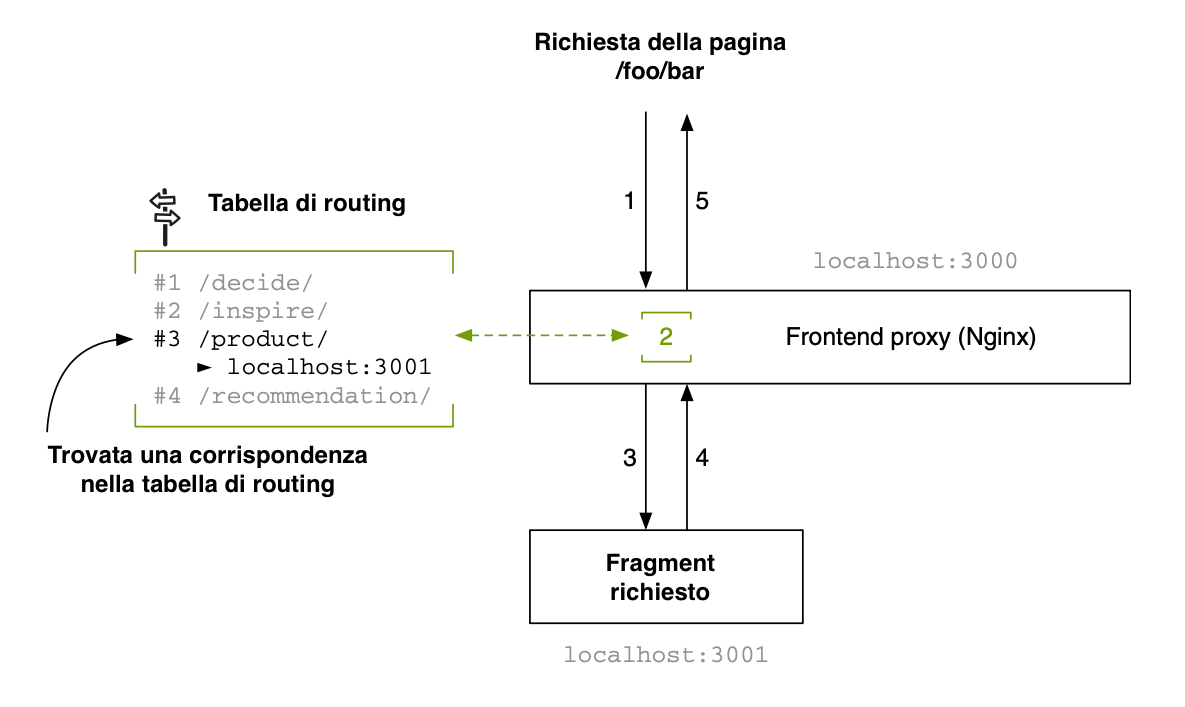
\includegraphics[width=140mm]{img/frontend proxy}
    \caption{  
        \textbf{1:} Il client apre l’ URL \emph{“/foo/bar”}. La richiesta raggiunge il frontend proxy;
        \textbf{2:} Il frontend proxy confronta il path \emph{“/foo/bar/“} con la propria tabella di routing, con corrispondenza in prossimità della regola i;
        \textbf{3:} Il frontend proxy passa la richiesta al fragment associato;
        \textbf{4:} Il fragment genera una risposta e la ritorna al frontdend proxy;
        \textbf{5:} La risposta arriva infine al client;
   }
  \end{figure}


\pagebreak

\section{Composizione Server-side}
Si suppone di lavorare ad un progetto microfrontend incentrato principalmente su contenuti e informazioni, senza particolari componenti logiche al suo interno.
Un esempio di sito incentrato sulle informazioni(anche detto \emph{content-centric}) è Wikipedia, le sue caratteristiche principali sono:
\begin{itemize}
    \item Tempi brevi di caricamento delle pagine
    \item Ottimizzazione per motori di ricerca
    \item Assenza di particolari contenuti basati su un interazione continua con l'utente
\end{itemize}

Si introduce quindi la \textbf{composizione server-side}, che va incontro alle richieste di un sito content-centric come Wikipedia.

La composizione dei fragment viene eseguita da un servizio che risiede nel server web, il client quindi riceve la pagina già completata.

Come nel caso degli iframes, i team che producono i fragments devono 
fornire al team che gestisce la pagina ospitante l'URL del loro codice HTML.

Il team della pagina ospitante userà delle direttive 
per richiedere al server di aggiungere il codice di markup degli altri team in un preciso posto della schermata.

Un esempio di servizio di composizione è la funzione \textbf{SSI} (Server-Side Includes) di \textbf{Nginx}:

\subsection{Server-Side Includes}

Nginx, il popolare web server che serve circa il 21\% dei siti internet\cite{nginx}, contiene il modulo \emph{ngx-http-ssi-module} che processa i comandi SSI.
 I comandi SSI sono istruzioni
inserite nelle pagine HTML della pagina ospitante. Un'istruzione SSI appare nella seguente sintassi:

   \begin{center}
    \verb|<!--#include virtual="url/da/includere -->|
   \end{center}

Quando il webserver legge la direttiva, effettua le seguenti operazioni:

\begin{figure}[H]
    \centering
    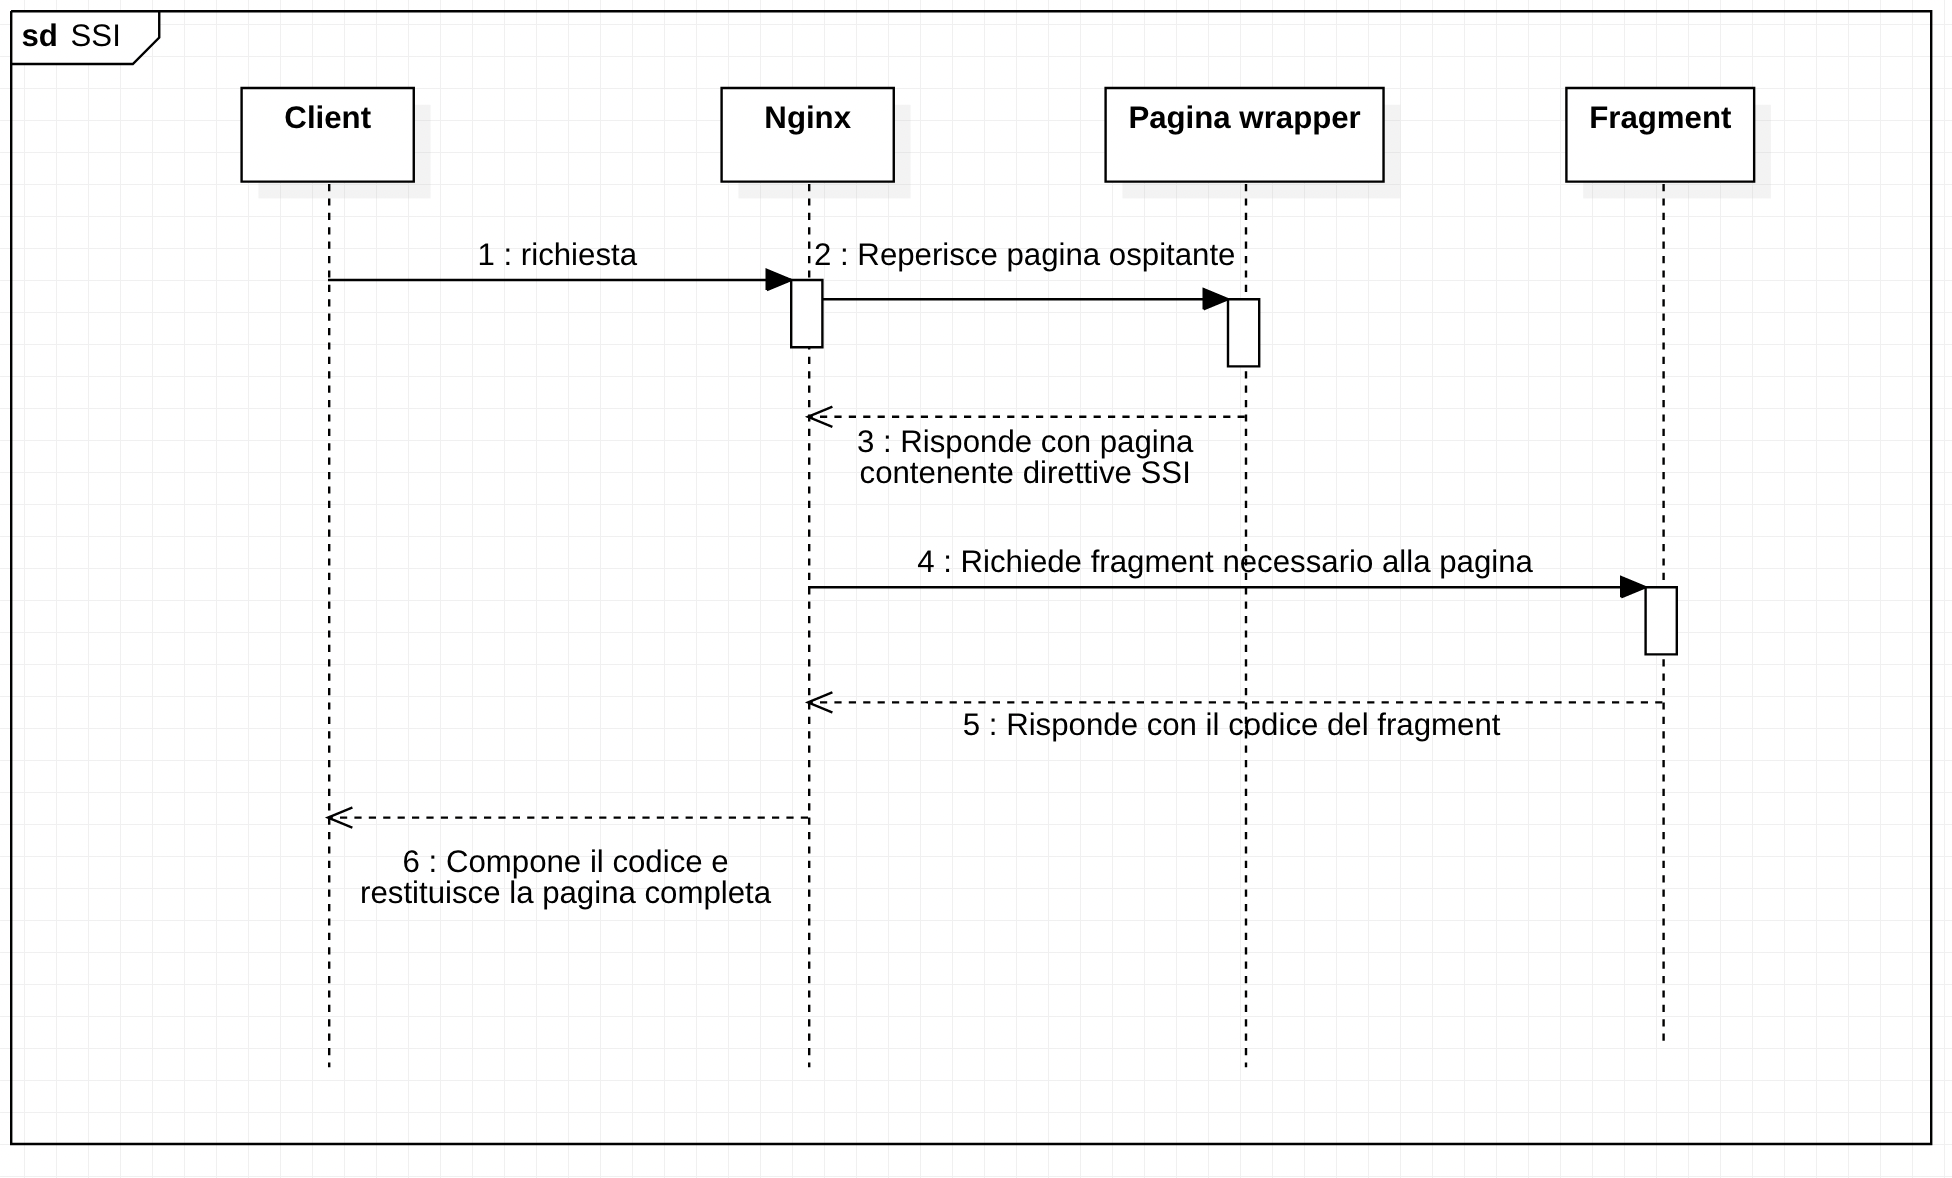
\includegraphics[width=140mm]{img/SSI sequence}
    \caption{ 
    \textbf{1:} Il client effettua la richiesta della pagina
    \textbf{2:} Il webserver accetta la richiesta e verifica la presenza di eventuali direttive SSI
    \textbf{3:} Le direttive trovate vengono sostituite con il codice di markup reperibile all'url dell'attributo "virtual"
    \textbf{4:} Il client riceve la pagina completa
    }
  \end{figure}


Le prestazioni dell'operazione di composizione sono nettamente migliorate rispetto ad iframes, 
in quanto il client riceve la pagina già completa, effettuando un solo handshake HTML, indipendentemente dal numero
di fragment ospitati nella pagina. Inoltre i motori di ricerca possono profilare anche il contenuto dei fragments.

\subsubsection{Modalità di caricamento dei fragments}
Al contrario della soluzione con iframes, lo scorretto caricamento di un fragment può rallentare o addirittura bloccare 
il caricamento dell'intera pagina. Il webserver infatti prima di restituire la pagina aspetta di avere tutti  i suoi componenti.
La proprietà di Nginx chiamata \emph{proxy read timeout} permette di fissare un tempo massimo per il quale il webserver 
può aspettare un fragment.
\\\\
Nel caso in cui il webserver non riesca a caricare un fragment esiste il comando SSI \textbf{stub}.
Si utilizza la direttiva \emph{block} che sostiuirà il fragment caricato senza successo con del codice HTML di riserva.
Il nuovo \emph{include} contiene l'attributo stub, che ha il riferimento al block corrispondente, nel caso non dovesse non andare
a buon fine la richiesta.
\\

\verb|<!--# block name="fallback" -->|\linebreak
\verb|      <a href="/page"> Link</a>|\linebreak
\verb|    <!--# endblock -->|\linebreak
\verb|          <!--#include|\linebreak
\verb|              virtual="/link/to/page"|\linebreak
\verb|              stub="fallback" -->|\linebreak


Quando Nginx deve scaricare più fragments, effettua i caricamenti in parallelo.
Solo quando l'ultimo fragment viene scaricato,la pagina viene composta e inviata al client.
\\
Il tempo di risposta dell'intera pagina è chiamato \textbf{time to first byte} (TTFB) ed è definito 
come il tempo necessario per generare l’HTML della pagina, sommato al tempo di caricamento del fragment più lento.

E' possibile anche annidare fragments, ma non è consigliato, in quanto si 
interrompe la parallelizzazione dei caricamenti e si rallenta la composizione della pagina.
\begin{figure}[H]
    \centering
    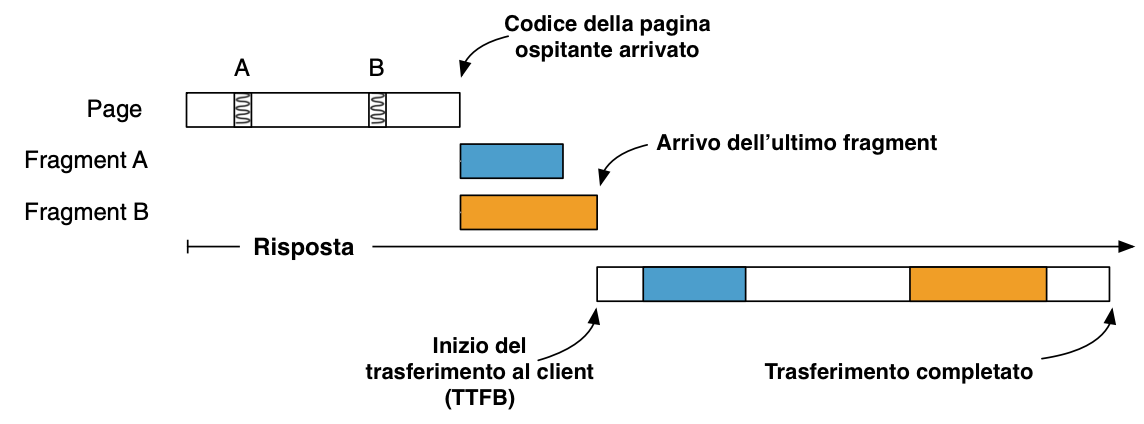
\includegraphics[width=140mm]{img/ssi parallelo}
    \caption{Sequenza temporale della composizione di fragment in parallelo con SSI}
  \end{figure}

\subsubsection{Caricamento differito}
In genere si ottimizza il caricamento della pagina effettuando una composizione server-side per la sua parte principale,
 la cosiddetta \emph{viewport}, le componenti secondarie invece è preferibile comporle lato client, con 
delle chiamate Ajax, utilizzando la metodologia descritta precedentemente. Questa tecnica si chiama caricamento differito, o \textbf{lazy loading}.
\\\\
\subsubsection{Alternative a SSI}
Il webserver con SSI, invia la pagina al client solo quando questa è stata completamente composta.
Il servizio di composizione \textbf{ESI} presente nel webserver Vernish invece attua l'\emph{invio parziale},
 ovvero inizia a restituire parti di pagina anche prima che questa venga completamente assemblata, 
 l'utente in questo modo potrà vedere informazioni, anche se non complete, in tempi più brevi.
\\
Esistono altre soluzioni, come quella sviluppata dalla società di fashion e-commerce Zalando, chiamata Zalando Tailor.
L'azienda migrò infatti il loro portale dall'approccio monolitico a quello microfrontend, utilizzando una composizione
server-side. Per via della grande dimensione del sito web, il team Zalando ha avviato il progetto Tailor, che ha poi portato ad un rilascio 
ufficiale con licenza libera. Tailor consiste in una libreria Node.js, reperibile nel pacchetto NPM \emph{node-tailor}.

Tailor riesce ad avere prestazioni migliori rispetto all'invio parziale, facendo in modo di iniziare a inviare parti di pagina al client,
ancora prima che il server abbia finito di scaricare l'intera pagina ospitante.

\pagebreak
\section{Composizione Client-side}
Ci sono dei siti web che non hanno principalmente uno scopo informativo, ma funzionale, ovvero rispondono all'input dell'utente
e rilasciano un output influenzato da tale input. Questi siti web vengono detti \emph{behavior-centric}, cioè 
incentrati su un comportamento o funzionalità.
Il modo più indicato per chiamarli non è siti web ma web apps, applicazioni web.
Una web app è ad esempio Google Meet, raggiungibile dall'URL https://meet.google.com.
Questo non è un sito che veicola principalmente informazioni, ma bensì offre un servizio all'utente: permette a due o più persone di 
interloquire, tramite scambio di segnali audiovisivi. Per fare in modo di reagire
all input degli utenti, le webapp cambiano il loro codice HTML nel browser, e inoltre permettono 
di cambiare pagina, e quindi anche URL, senza effettuare alcuna richiesta al webserver.
Sono disponibili agli sviluppatori numerosi framework per realizzare webapps, come React.js, Angular e Vue.js.
Seguendo un approccio monolitico dovremmo scegliere uno di questi framework ed essere costretti a farlo utilizzare
a tutti i team che lavorano al progetto. Al contrario, con l'approccio microfrontend, si da libertà ad ogni team
di scegliere autonomamente la soluzione migliore e di mantenerla aggiornata.
Grazie agli \textbf{web components}, i team possono realizzare dei fragments con qualsiasi tecnologia a loro disposizione e 
farli operare con il resto della pagina.



\subsection{Web Components}
Gli web components consentono di creare nuovi elementi HTML personalizzati ( Custom Elements), riutilizzabili e incapsulati
da utilizzare in siti e web app \cite{webcomponents}.

Custom Elements è un insieme di API Javascript che consentono di definire elementi HTML personalizzati, che includono istruzioni CSS e JS.
Ogni custom element è dichiarato nell' oggetto \emph{CustomElementRegistry}.
\linebreak

All'interno di un web component può essere incapsulato elementi di stile e componenti logiche, senza influenzare
la parte restante del DOM (Document Object Model), questo grazie alla \emph{shadow DOM}:
\subsubsection{Shadow DOM}
Sappiamo che il DOM (Document Object Model) è un albero di oggetti creato alla fine del caricamento di ogni pagina web, che 
permette di accedere dinamicamente e aggiornare il contenuto, la struttura e lo stile di un documento.\cite{dom}
Possiamo annettere alla struttura del DOM, un numero arbitrario di \emph{shadow trees}, 
o alberi ombra, questi con i loro elementi e il proprio design hanno una radice, detta  \emph{shadow root}.
La shadow root è sempre annessa ad un \emph{shadow host} che risiede nel DOM o in un altro shadow tree.

Grazie alla Shadow DOM è possibile gestire singoli elementi di un progetto web in modo indipendente rispetto al resto del sito.
Dentro la shadow DOM è possibile gestire contenuti in maniera del tutto indipendente rispetto alle istruzioni di design o dalle strutture
valide globalmente nel resto del progetto.

Questo aumenta la robustezza del microfrontend, garantendo isolamento.
\linebreak
\linebreak
Un altro elemento importante che sta alla base dei web components è il concetto di \textbf{template HTML}: 
un modo per creare codice HTML non ancora visualizzato sulla pagina, che può essere istanziato una o più volte 
durante il runtime grazie a codice javascript.



\subsection{Comunicazione tra fragments}
I fragment possono aver bisogno di ricevere dalla pagina 
ospitante delle informazioni di contesto, come ad esempio la lingua, 
la regione geografica, o il nome dell'utente recuperata da un database.
Gli attributi dei custom element possono fungere da mezzo di comunicazione per inviare
informazioni dalla pagina al fragment.
I custom elements, con i quali sono implementati gli web components, forniscono agli sviluppatori 
una serie di metodi che interessano momenti del loro ciclo di vita:
\begin{itemize}
    \item \textbf{connectedCallback}: invocato quando il custom element viene inserito nel DOM della pagina 
    \item \textbf{disconnectedCallback}: invocato quando il custom element viene rimosso dal DOM
    \item \textbf{adoptedCallback}: invocato quando l'elemento viene spostato da un documento ad un altro
    \item \textbf{attributeChangedCallback}: invocato quando un qualsiasi attributo del documento cambia
\end{itemize}

Si può quindi utilizzare il metodo \emph{attributeChangedCallback} per far reagire il fragment in risposta ad un
attributo cambiato.


Per quanto riguarda la comunicazione da un fragment alla pagina, è possibile utilizzare 
l'API nativa \textbf{CustomEvents}, disponibile in tutti i moderni browsers.
Permette di emettere eventi personalizzati allo stesso modo di come funzionano gli eventi standard \emph{click} o \emph{change}.

Per far si che il colloquio vada a buon fine, il team che gestisce il fragment deve comunicare a quello che gestisce la pagina
il nome dell'evento.

\pagebreak

Analizziamo adesso le diverse strategie per far comunicare due fragment ospitati sulla stessa pagina:

\begin{itemize}
    \item \textbf{Comunicazione diretta}: consiste nel chiamare direttamente il metodo del fragment
    interessato, secondo il principio che qualsiasi fragment ha accesso all'intero DOM della pagina.
    Questo metodo è altamente sconsigliato, perchè introduce un \textbf{forte accoppiamento}
    \item \textbf{comunicazione tramite pagina ospitante}: si usa la pagina ospitante come tramite del messaggio,
    utilizzando le tecniche prima viste, si emette un evento dal fragment A, si riceve nella pagina, e si inoltra ad un attributo 
    del fragment B.
    \item \textbf{Broadcast Channel API}: la Broadcast channel API permette la comunicazione 
    tra elementi del browser della stessa \emph{origin}, ovvero con hostname, e porta uguali. 
    Si basa sul meccanismo publish/subscribe.
    Vengono instaurati dei canali nei quali vengono pubblicati messaggi (\emph{publish}), 
    che riceveranno solo i fragment che si sottoscrivono a tale canale(\emph{subscribe}).
    Questa soluzione riduce al minimo l'accoppiamento tra i vari fragments.
    Broadcast channel API verrà approfondito successivamente.
\end{itemize}

E' importante che le comunicazioni tra i fragemnt siano minime e che interessino dati semplici, in quanto
un eccessivo accoppiamento tra due oggetti può significare un inesatto confine tra due team.

\pagebreak
\subsection{Routing Client-Side }
La maggior parte dei framework client come Angular o React hanno al loro interno un servizio che permette di
effettuare routing, attuando una navigazione tra differenti pagine senza fare una completa richiesta al server.
In questo modo le webapp con un routing lato client appaiono all'utente più reattive e offrono una migliore esperienza.
Queste webapp vengono chiamate Single Page Applications, o SPA.

Si deve innanzi tutto distinguere due tipi di navigazione:
\begin{itemize}
    \item \textbf{Hard navigation}: il browser durante la navigazione carica completamente il codice HTML dal server
    \item \textbf{Soft navigation}: la transizione avviene lato client, in questo modo non si richiede la pagina completa,
     ma solo alcuni dati, che vengono caricati dal server tramite una API Javascript
\end{itemize}

Di conseguenza i team possono scegliere autonomamente il tipo di navigazione.
Si può trovare una webapp con una hard navigation in tutte le pagine, anche in quelle interne di un team,
oppure quella che viene chiamata \emph{linked SPA}, con hard navigation per passare da una pagina posseduta da un team ad un altro
e soft navigation per le pagine dello stesso team.

In entrambe queste soluzioni l'unico dato che deve essere condiviso tra i team, il cosiddetto contratto, consiste 
unicamente nell' URL delle pagine. Questo garantisce una grande autonomia tra team e un alto disaccoppiamento.

Il passo successivo è quello di rendere l'esperienza utente più fluida, introducendo una soft navigation anche tra pagine di team 
diversi. Per fare ciò è necessario un infrastruttura condivisa, chiamata \emph{Application Shell}.


\subsubsection{Application Shell}
L' Application Shell, o App Shell, è un app che sta alla base di tutti i microfrontend. Questa si occupa di instradare le
richieste e di visualizzare nella pagina HTML il microfrontend giusto. Di solito risiede nella pagina principale( index.html) ed essendo
condivisa con tutti gli altri elementi deve essere mantenuta il più semplice possibile.
Di solito viene incluso nell'app shell le informazioni di contesto o di autenticazione, utili a tutti i microfrontend.

Un team sarà responsabile della sua manutenzione e dovrà essere a conoscenza del nome dei custom element con i quali gli altri team forniscono
le loro web app.
Inoltre l'app shell, per instradare correttamente tutti gli indirizzi, deve essere a conoscenza degli url di tutte le pagine di ogni team.
Questo obbgliga i team a notificare l'app shell di qualsiasi aggiunta o rimozione di pagine nel loro progetto.

Con il \textbf{routing a due livelli} si porta l'app shell in una posizione più neutrale e si diminuisce l'accoppiamento tra questa e gli altri microfrontend.
\subsubsection{Routing a due livelli}
Risolviamo il problema facendo instradare le pagine all'app shell soltanto secondo il team di provenienza.
Ogni team avrà un router interno che assegnerà all'url in arrivo la pagina corrispondente.
Per identificare chiaramente il team, si utilizza un prefisso nell'URL.

In questo modo l'app shell viene cambiata solo se si aggiunge un nuovo team o si vuole cambiare il nome dei prefissi.



\pagebreak
\section{Universal Rendering}
Dopo aver visto come comporre microfrontend in maniera server-side e client-side, vediamo come combinare queste due tecniche
per capire quali vantaggi possono apportare ad un progetto web.
Il concetto che sta alla base dell' universal rendering è il seguente:
' Avere un'unica sorgente di codice che è possibile renderizzare sia sul server che su un client ' \cite{ssr}

Supponiamo di realizzare una pagina per un e-commerce di vestiti.
Nella pagina sarà presente l'elemento più importante, quello che riesce a monetizzare la visita di un utente: il pulsante "compra".
Il bottone "compra" è un microfrontend con stili e funzioni logiche gestite da un team specializzato, racchiuso in un web component.
Data l'estrema priorità di avere visualizzato e funzionante il prima possibile il bottone, il team non si accontenta di una client-side composition,
in quanto per dispositivi lenti,con internet scarso, o senza il supporto di javascript potrebbe non funzionare la composizione dell'elemento, 
il che porterebbe ad un mancato guadagno per il sito.

Una possibile soluzione è utilizzare la Server Side Integration per creare il bottone, prima di consegnare la pagina al client, in questo modo l'elemento 
verrà subito visualizzato. Successivamente il client attuerà la composizione lato client e il bottone sarà completamente stilizzato.

In questo modo l'utente può comprare il prodotto appena la pagina viene scaricata sul browser.

Vediamo i casi in cui è utile la Universal Rendering: \cite{angularUniversal}
\begin{itemize}
    \item \textbf{Ottimizzazione SEO}: è necessario per i crawler dei motori di ricerca avere una versione statica del sito web
    facilmente navigabile senza l'utilizzo di javascript. In questo modo ogni URL ritorna un'anteprima fedele e completa della pagina
    \item \textbf{Performance in dispositivi lenti}: alcuni dispositivi poco potenti o non aggiornati potrebbero non supportare correttamente
    Javascript, è quindi utile avere una versione del sito funzionante senza l'uso di scripts.
    \item \textbf{Velocità di caricamento}: l'utente ha immediatamente una versione statica del sito completamente navigabile, che successivamente
    con la composizione client-side diventa anche completamente interattiva. Questo è fondamentale per le landing page, che hanno l'obiettivo di convertire il più 
    possibile le visite
\end{itemize}


In conclusione universal rendering è la soluzione più complessa di composizione, ma anche l'unica che riesce a unire la velocità di caricamento delle pagine server-rendered
e l'estrema velocità di risposta all'input delle pagine client-rendered.

Una SPA che ha elementi di server side rendering viene chiamata \emph{universal unified SPA}.

